\chapter{Background} %Chapter title 

 

There are four primary areas where the extant literature must be analyzed. First, it is important to understand the distinction between homelessness and housing insecurity. Next, it is necessary to take a multi-disciplinary look at each pillar of the 4 Cs of housing insecurity. Third is the unique challenges that rural areas face in order to better inform the theoretical framework. Finally, the theoretical foundations of the methods and their previous applications in the study of housing insecurity tie together the literature with the methods used. These four aspects form the theoretical basis for exploring rural housing insecurity. 

 

\section{\textit{Housing Insecurity}} 

 

Housing insecurity is a term that stems from the shift in homelessness research from focusing on only the housed and the unhoused. \citet{deluca_housing_2022} argue that the term housing insecurity is a more dynamic concept than the traditional housed and unhoused binary. "Housing insecurity operates through multiple mechanisms-including material hardship, stress, environmental and infectious disease exposures, social network disruption and barriers to healthcare- to produce adverse health outcomes over the life course" \citep[759]{leifheit_building_2022}. Homelessness is generally attributed to poverty and a lack of access to affordable housing \citep{national_coalition_for_the_homeless_rural_2009}. As researchers shifted away from the housed and unhoused binary, identifying characteristics that distinguish the housed from the unhoused led to identifying factors that occur on the path to homelessness \citep{phelan_social_2010}. The identification of these factors likely contributed to the rise of housing insecurity as a concept and as a field of study. \citet{deluca_housing_2022} argue that housing insecurity may be a more useful term than the housed and unhoused binary because it acknowledges housing hardship and housing risk as a continuum that affects a wider section of the population than literal homelessness. One issue with the study of housing insecurity is that, like rurality, a wide variety of definitions are used. Cox et al. (2019) analyzed 106 studies and found that current approaches to housing insecurity have three major issues: a lack of a uniform definition, it is often applied as an underdeveloped concept, and it is often measured inconsistently. An explanation for this variation is that housing insecurity operates through a variety of mechanisms, a relationship the 4 Cs model encapsulates \citep{leifheit_building_2022}. Rather than giving a strict definition, it may be more beneficial to look at the dimensions of housing insecurity. \citet{cox_road_2019} identifies seven dimensions of housing insecurity: housing stability, housing affordability, housing quality, housing safety, neighborhood safety, neighborhood quality, and literal homelessness. To adequately address housing insecurity, it is necessary to have a theoretical framework that can encompass these different dimensions to avoid these pitfalls.  

 

\section{\textit{The 4 Cs of Housing Insecurity}} 

 

To understand housing insecurity in the context of the 4 Cs framework, the following subsections detail each pillar of housing insecurity under the model proposed by \citet{hernandez_housing_2019}. As each pillar forms a web rather than separate pieces, there is a significant amount of overlap between pillars. The pillars meet the dimensions identified by \citet{cox_road_2019}: housing stability (consistency), housing affordability (cost), housing quality/ housing safety (conditions), and neighborhood safety/ neighborhood quality (context). % More on the 4 Cs  

\subsection{\textit{Cost}} 

Housing affordability is generally conceived as the amount of a household's budget that goes to housing, including rent or mortgage payments, utilities, and other expenses. A cost-to-income ratio is the most common way of measuring housing affordability. It is difficult to determine one number that determines when a household is spending too much on housing. The threshold for housing affordability has varied between 25 and 50 percent with the current standard set at 30 percent \citep{kropczynski_insights_2012}. Today, Housing is considered affordable if the household spends less than 30 percent of its income on housing, and 50 percent or more is considered a high-cost burden (\citealp{braveman_housing_2011}; \citealp{swope_housing_2020}; \citealp{weicher_housing_2006}). Inherent to a cost-to-income ratio is the understanding that there are other expenses necessary for survival \citep{herbert_measuring_2018}.  

%Housing costs are determined by the rate of household formation and household attrition \citep{pendall_future_2016}.  

Housing affordability affects individuals, families, and communities while access is largely determined by their demographic characteristics (\citealp{braveman_housing_2011}; \citealp{yadavalli_comprehensive_2020}). Housing affordability is directly related to residential stability and has the potential to harm those being forced to move, the community they are leaving, and the community they are entering \citep{desmond_forced_2015}. Access to affordable housing affects the physical and material comfort of communities and individuals. If a household cannot afford to live in their current place, they may be forced to relocate seeking more affordable housing voluntarily or through eviction and foreclosure. If too much of a household’s money goes to housing, they may be forced to go without other necessities \citep{herbert_measuring_2018}. Those with high housing costs may also experience food insecurity as food is often considered a flexible expense while housing is a fixed expense (\citealp{fletcher_assessing_2009}; \citealp{kropczynski_insights_2012}). This is only one area where low-income households may have to compromise to maintain their fixed housing costs. Housing is often the biggest expense for low-income families, forcing them to make trade-offs between housing and other necessities \citep{desmond_housing_2015}. The shortage of affordable housing drives lower-income families to substandard housing in worse neighborhoods \citep{braveman_housing_2011}. This creates the potential for a spiral where housing instability cannot be escaped due to the added costs of moving. \citet{kang_severe_2021} characterizes housing instability as a by-product of the affordable housing shortage wherein households can be destabilized by minor financial shocks. These factors can create a situation where housing costs lead to residential instability, which is linked to a variety of adverse conditions, especially in children and adolescents \citep{desmond_forced_2015}. Housing affordability is both influenced by and exerts influence on many other aspects of life, and its relationship to housing insecurity cannot be understated.  

 

\subsection{\textit{Conditions}} 

 

Internal housing conditions have been identified as a significant factor on health (\citealp{braveman_housing_2011}; \citealp{metzger_fair_2017}; \citealp{swope_housing_2020}). In one study, decent housing was found to be a more important determinant of health than education or income \citep{angel_housing_2014}. Previous environmental health research has identified five broad categories in which housing conditions contribute to adverse health effects: physical conditions, chemical conditions, biological conditions, building and equipment conditions, and social conditions \citep{jacobs_environmental_2011}. Links to an increase in disease have been tied to poverty, poor housing, and degraded environments reflecting the interconnectedness of housing insecurity issues \citep{rauh_housing_2008}. \citet{angel_housing_2014} found that the probability of facing a chronic disease increases when housing problems accumulate and that poor housing conditions quickly degrade subjective health. These problems are amplified in the modern world where individuals spend an estimated 90 percent of their time indoors \citep{palacios_impact_2021}. The relationship between housing conditions, poverty, and the range of factors that contribute to housing conditions emphasize the importance of viewing housing as a matter of health. Housing conditions also play a role in residential mobility as \citet{desmond_housing_2015} place decent housing and affordable housing as fundamentally connected and the previously mentioned rise in housing cost has not brought an increase in housing quality. The impacts of housing conditions on health means that adequate housing is a public health issue \citep{matte_housing_2000}. Despite housing conditions playing such a significant role in modern life, there is not a significant sense of communal benefit and responsibility when it comes to housing \citep{jacobs_environmental_2011}. Without a sense of communal benefit towards housing, this leaves marginalized populations that are more likely to be exposed to harmful housing conditions without community support \citep{swope_housing_2020}. Growing a sense of communal benefit towards housing would be beneficial for all aspects of housing.  

 

\subsection{\textit{Consistency}}  

% see Jaquet article  

Residential mobility is a complicated subject because, as a broad concept, it is conceived as a good thing. That one can pack up and go somewhere with more opportunity is considered a part of the American “mystique” \citep{molloy_internal_2011}. An average of 15 percent of Americans move every year and 25 percent move over two years \citep{bachmann_ins_2014}. Classic urban economic theories hold that households make trade-offs between proximity to jobs and housing prices \citep{hu_housing_2019}. This puts low-income households at a disadvantage as their access to jobs may be lower than their wealthier counterparts. Consistency plays an important role in the physical and social well-being of individuals, families, and communities. It has been linked to a variety of adverse conditions and affects the neighborhoods being entered and left. It has been identified as a more important predictor of community health than standard factors like poverty and racial composition (\citealp{desmond_forced_2015}; \citealp{desmond_housing_2016}; \citealp{rauh_housing_2008}). An important distinction must be made between voluntary and involuntary moves \citep{siskar_who_2019}. While most moves are voluntary, millions of low-income households struggle to maintain housing stability (\citealp{phinney_exploring_2013}; \citealp{kang_why_2019}). Besides voluntary relocations forced relocation can be triggered by foreclosure, eviction, and condemnation (\citealp{phinney_exploring_2013}; \citealp{siskar_who_2019}). It is linked to an increase in residential instability and households forced to move often end up in places with greater disadvantage and are more likely to face additional moves \citep{desmond_forced_2015-1}. One issue with the study of residential mobility is the limited scope of linked predictors \citep{kang_why_2019}. This limits our ability to analyze and reduce negative residential mobility. One group at a higher risk of housing instability are those who rent their housing. Renters are particularly vulnerable to relocating to worse neighborhoods than the ones they are exiting \citep{desmond_forced_2015}. Residential instability is closely related to housing affordability, housing conditions, and context. These relationships reinforce the idea that housing insecurity is an interconnected web. 

 

\subsection{\textit{Context}} 

% highlight what the “Context” “C” focuses on and then clearly state if you’re addressing all of the “Context” items the 2019 piece outlines and explain why you’re focusing on the “context” pieces you chose to focus on. I think those pieces are here, but can be made a bit clearer.  

Context revolves around neighborhood and community characteristics including demographics, green spaces, education, and healthcare among many other things. Context involves "the presence of positive or adverse health-relevant resources in the surrounding neighborhood" \citep[9]{swope_housing_2020}. This makes it difficult to capture context in its entirety due to its wide scope. To best encapsulate context with the available data, this thesis focuses on demographics, employment, housing type, and household factors as these have all been studied as matters related to housing insecurity that do not fall directly into the other pillars of housing insecurity. The following is an interdisciplinary review of how these selected factors affect housing insecurity.  

 

\subsubsection{\textit{Employment}} 

 

In the United States, the labor market is the result of cumulative individual behaviors including geographical migration and educational investments \citep{wiener_labor_2020}. The demand for labor is driven by firms, which must consider a wide variety of factors in deciding location \citep{partridge_persistent_2007}. In recent decades, the United States labor market has entered a risk regime job market where workers hold a greater share of the risk in an employment system without the perceived promise of security and stability which has become embedded in American social and political institutions \citep{lowe_perceived_2018}. It is agreed that the Fordist regime that brought unprecedented prosperity in the early 20\textsuperscript{th} century came to an end in the 1970s \citep{stockhammer_stylized_2008}. Since this shift, the productivity of the average worker has increased by 64.7 percent while hourly pay has only increased an average of 17.3 percent between 1979 and 2022 \citep{economic_policy_institute_productivity-pay_2022}. Over this same period, HUD data show that the median price of a new single-family home increased from \$60,600 (\$232,091 adjusted for inflation) in 1979 to \$369,800 in 2021 \citep{us_census_bureau_median_2023}. % I need to fix this date 

These shifts in the housing market are one of the underlying factors in the rise of the affordable housing shortage. As wages have failed to keep up with the price of housing, the current economic system under the risk regime places those with low incomes in a precarious situation for housing affordability and residential stability. %The Great Recession has had a lasting impact on the housing market within the United States. As the economic recovery did not benefit all households equally, wealth inequality has grown along both racial and ethnic lines \citep{kochhar_wealth_2014}. 

Employment insecurity and income inequality are two pressing issues the United States is facing that have serious impacts on communities. “Housing insecurity has risen in relative lockstep with employment insecurity” \citep[48]{desmond_housing_2016-1}. Economic conditions play a significant role in housing insecurity because adequate income is critical for all aspects of housing insecurity.  

 

 

One significant cause of employment insecurity is a lack of economic diversity, generally caused by a lack of economic development. \citet{sherrieb_measuring_2010} identify three key elements connected to economic development: the level of economic resources, the level of equality in resource distribution, and the level of diversity in economic resources. Economic development alongside demographic change in rural areas have been linked to the quality and condition of local housing infrastructure \citep{barcus_heterogeneity_2011}. How policies shape economic development has a direct effect on the overall housing insecurity risk of rural communities. Amid the recent major economic shifts, globalization and shifting employment sectors play a critical role in the development path of communities which has an inherent effect on the people who live there \citep{harrison_spatial_2019}. Demonstrating the interconnectedness of communities, regional economic development in one area can encourage economic stability of its neighboring regions as well so it is important to view communities as interrelated rather than separate entities \citep{chen_economic_2018}. \citet{deller_spatial_2016} highlights the importance of economic diversity, a vital aspect of economic development, finding that more diverse economies enhance economic stability. As an insulator against economic instability, employment diversity is a key factor that policymakers and scholars should consider as part of a holistic approach to housing insecurity.  

 

\subsubsection{\textit{Housing, race, education, and poverty}} 

 

Housing is affected by a variety of social, political, and economic factors. “The ability of residents to access affordable housing, whether renting or buying, is in large part determined by their demographic characteristics, such as income, race, age, and educational attainment” \citep[115]{yadavalli_comprehensive_2020}. While unpredictable events may narrow the disparities, “As a rule, a household’s vulnerability to displacement should be shaped in a predictable fashion by those characteristics that define its members’ position in the [social] stratification system” \citep[5]{lee_forced_2020}. This vulnerability is driven by a combination of individual and socio-demographic factors. One major factor that has made minorities vulnerable to housing insecurity is discrimination in housing. Although the federal government took a direct interest in promoting home ownership in 1933, racial discrimination in the housing market was not outlawed until 1968 and enforcement of the law remained difficult until the Fair Housing Act of 1988 \citep{sharp_emerging_2014}. For example, the practice of redlining made it difficult for African Americans to receive mortgages under federal aid programs and created racial segregation that can still be seen today. At the county level, the probability of living in affordable housing decreases as the white population decreases (Brooks, 2022). In addition to racial segregation, income segregation must be considered for a holistic discussion of housing insecurity. A high concentration of poverty may exacerbate housing conditions issues due to a lack of revenue to maintain the necessary services at the household and local government levels. Minorities are also at a disadvantage in income segregation with poor whites being less segregated from their non-poor counterparts \citep{lichter_ruralurban_2021}. As a home is often a household's greatest source of wealth, the disadvantages minorities have in terms of housing are compounded as social and economic inequality are reproduced as these disparities continue \citep{krivo_housing_2004}. These sources of inequity are an important part of a holistic approach to housing insecurity.  

 

% add something on rural gentrification and native American reservations in rural areas  

 

\subsubsection{\textit{Housing Type}}  

 

While owning a home is considered a part of the “American Dream,” many households rent their housing by choice or by necessity. While the many benefits of home ownership portray it as a means to a better life, renting is not inherently bad and may provide better opportunities for households that can afford it, but there are many potentially destabilizing consequences of high-cost renting \citep{drew_believing_2014}. Nationally, the median rent in a poor neighborhood is higher compared to a middle-class or affluent neighborhood after regular expenses are deducted despite property values typically being much higher in middle-class or affluent neighborhoods \citep{desmond_poor_2019}. This creates a compounding factor for the previously mentioned disparities in home ownership. Increases in household wealth and secured debt were found to decrease the likelihood of homeowners becoming renters and vice versa \citep{anderson_effect_2021}. Renters with high-cost housing are unable to increase household wealth through their means of housing. In addition to whether one rents or owns a home, the type of home can play a significant role in housing insecurity. Of particular concern is unconventional housing which includes dwellings not considered long-term habitation including RVs/ campers, vans, and boats. These unconventional forms of housing may keep people off the streets, but they are not always a stable mode of housing. For RV and camper living, people who are undocumented or are unable to keep up with legal or maintenance costs for vehicles end up losing their housing, making an already vulnerable population more vulnerable \citep{wakin_not_2005}. In rural areas, mobile homes are often seen as an affordable option, but they come with certain risks not as common in traditional housing. Structural problems like poor construction and risks of air pollution and fire create a unique problem \citep{mactavish_policy_2006}. Mobile homes also carry a unique set of circumstances that may put households at a greater risk of housing insecurity and are found frequently in rural areas \citep{mactavish_wrong_2007}. Individuals who rent or own mobile homes, unconventional housing, face high rental costs or high mortgage costs are at a heightened risk of housing insecurity in rural areas and should be taken into consideration.  

 

 

\subsubsection{\textit{Household Factors}} 

In his first State of the Union address, President Lyndon B. Johnson asked Congress to declare an “unconditional war on poverty… not only to relieve the symptom of poverty but to cure it and, above all, to prevent it” \citep{the_american_presidency_project_annual_nodate}. Since then, the patchwork of programs regulated at the federal, state, and local levels has expanded. A large part of the federal government's growth in the late 20\textsuperscript{th} century is from the expansion of social welfare spending \citep{fishback_social_2020}. Today, the primary mechanism of income distribution is what \citet{berkowitz_gaps_2023} refer to as the “factor payment system” in which those who work and those who own the means of production and one’s relation to this system and the labor market are closely related to one’s poverty risk. To alleviate this poverty risk, social programs that utilize different mechanisms are available to those who qualify. These mechanisms can be divided into categorical and income-targeted policy designs, alongside decentralization, where some receive benefits based on “demographically defined, categorical eligibility structures” and others enjoy standardized federal assistance through social insurance with some qualifying for income-based or “means-tested” programs \citep{bruch_poverty_2023}. Households must fall below certain income and asset thresholds to qualify for means-tested programs \citep{rank_welfare_2002}. For housing, there is a wide variety of housing policies and programs aimed at low-income individuals. These take the shape of voucher programs by subsidizing privately held property although some recipients live in public housing \citep{kim_housing_2017}. For rural areas, the U.S. Department of Agriculture (USDA) has a variety of programs aimed at improving living conditions in rural areas including direct or guaranteed loans for single or multi-family housing, and infrastructure programs for water, electricity, and telecommunications \citep{us_department_of_agriculture_usda_2023}. Transportation plays a large role in social and economic life. Access to everything from education to healthcare depends on the infrastructure and the ability to use available means of transportation. Rural areas often do not have public transportation, leading residents to depend more on automobiles. An analysis of 2009 National Household Travel Survey data found that 72 percent of households with a yearly income of \$20,000 have access to a household vehicle compared to over 97 percent of households making \$50,000 \citep{blumenberg_automobile_2012}. This is another instance where opportunity is dependent on a household's income. Automobile ownership can be a crucial factor in avoiding residential instability \citep{kang_why_2019}. This concerns rural areas without public transportation where distances may be too far or too dangerous for alternate means of transportation due to a lack of proper road infrastructure, limiting access to adequate employment and opportunity. Areas at a high risk of housing insecurity are likely to exhibit many of these factors and they play a significant part in the context of housing.  

% talk about aging population 

 

\section{\textit{Challenges for Rural Areas}}  

 

Rurality is often defined simply as not being urban \citep{robertson_rural_2007}. Defining rural areas in contrast to urban areas largely excludes the variation between rural areas. The Census Bureau defines metro areas as urban areas of 50,000 people or more, and urban clusters of 2,500 to 49,999 people with all other areas classified as rural; the Office of Management and Budget defines metro areas as urban cores with populations of 50,000 or more people, micro areas as urban cores of 10,000 to 49,999 people where micro areas and counties outside of metro and micro areas are considered rural \citep{health_resources__services_administration_defining_2022}. Several measures consider rurality a spectrum, such as the Rural-Urban Commuting Area Codes (RUCA) used in this research. RUCA codes form an urban-rural scale ranging from 1 to 10, accounting for population, density, urbanization, and commuting \citep{usda_economic_research_service_rural-urban_2023}. Choosing an appropriate set of RUCA codes can more adequately capture the number of rural people that live in areas classified as urban identified by \citet{isserman_national_2005}. Improperly classifying rural areas as urban or wrapping all rural areas into a blanket group reduces ability to address housing insecurity appropriately \citep{yousey_defining_2018}.  

 

Part of the blanket construct of rural areas is that they are cheaper to live in. However, \citet{kurre_is_2003} notes that there is relatively little systematic data that supports this presumption. \citet{zimmerman_does_2008} found no consistent pattern of lower prices across rural counties in Pennsylvania. Rural areas face the same low per capita income and poverty problems faced by urban areas \citep{castle_place_2011}. While the dollar amount paid for housing may be lower, given the different socio-economic circumstances of rural areas, housing costs alone may not fully encapsulate the situation \citep{kropczynski_insights_2012}. Although there is limited research on homelessness in rural areas, previous research has documented the unique struggles of rural areas that should be addressed in a discussion on rural housing insecurity. First, scholars have identified both pockets of prosperity and pockets of deep poverty in rural areas. Concentrated poverty is "often the manifestation of an interactive and inter-generational dynamic between structural changes that restrict economic opportunities and the emergence of populations with characteristics that put members at a relatively high risk of poverty" \citep[7]{thiede_spatial_2018}.  

Poverty is acknowledged more in urban areas, but poverty rates are highest in both remote rural counties and in cities (\citealp{miller_persistent_2003}; \citealp{crandall_local_2004}). Persistent poverty, typically defined as poverty levels above 20 percent, is geographically concentrated in rural regions \citep{crandall_local_2004}. In 2010, the poverty rate among the rural population was higher than that of the nation overall \citep{burton_inequality_2013}. \citet{lichter_rural_2011} found that 40.5 percent of high-poverty places are in high-poverty counties for non-metro areas and the poor and non-poor are becoming increasingly segregated, with higher concentrated poverty among minorities. A cluster analysis found 3,017 places with poverty rates around 20 percent above the national average that account for about 5 percent of the nation's population and almost 87 percent of this population lives in rural areas \citep{peters_typology_2009}. \citet{lichter_changing_2007} found that 85 percent of the nearly 500 counties with poverty rates over 20 percent and the 12 counties with poverty rates over 40 percent are in non-metro areas. The areas with persistent poverty have some similar characteristics: they have primarily agricultural or resource-based economies, reduced employment opportunities due to economic changes, or gentrification is making living costs unaffordable for many people \citep{robertson_rural_2007}. 

One potential explanation for the persistent effects of poverty in rural areas is the isolation from schools, services, social interactions, and labor market resources \citep{canto_rural_2014}. Isolation stems from limited ease of travel or access to nearby markets and population centers which can hinder economic development, meaning that greater geographic isolation is associated with both lower income and greater poverty rates \citep{blank_poverty_2005}.  

Looking only at poverty does not tell the full story of rural areas. There are more than 300 rural counties spread across the nation that are more "prosperous" than the rest of the nation based on measures spanning education, housing, poverty, and unemployment \citep{isserman_why_2009}. This highlights the need for an approach to rural areas that is relative rather than absolute. \citet{metzger_fair_2017} highlight the tendency for Americans to segregate themselves not only based on race but on class too. A tendency for the rich and the poor to cluster around themselves could explain these findings in rural areas. This spatial inequality is critical to understanding rural poverty \citep{thiede_spatial_2018}. Spatial inequality expands concerns with stratification into the realm of geographic space \citep{lobao_spatial_2002}. In rural areas where location determines many aspects of the community constructed on top of it, researchers cannot ignore the implications of spatial inequality. The presence of both highly prosperous and highly impoverished rural areas indicates a need for a better understanding of the role of spatial inequality in rural areas.  

 

Another problem that rural areas are facing is a growing economic divide between urban and rural areas \citep{bjerke_mover_2019}. Rural communities have been hit hard by economic changes in recent decades, driven by the transition from a production to a consumption-based economy \citep{pendall_future_2016}. During this shift, employment became increasingly scarce for agricultural workers \citep{kropczynski_insights_2012}. Today, manufacturing is responsible for 21 percent of rural non-agricultural earnings \citep{low_rural_2017}. Economic development is therefore a fundamental issue to rural areas. While manufacturing has grown, the majority of counties that experienced manufacturing employment growth between 2001 and 2015 had low levels of growth in terms of total employment \citep{low_rural_2017}. \citet{blank_poverty_2005} note that rural areas often have more limited job opportunities and are more likely to rely on one industry rather than having a diversified economy. Preventing the amelioration of problems facing rural areas is the relatively uncoordinated approach to rural development that has occurred despite the active role the federal government has played in it \citep{wilson_rural_2016}. As a result, some rural regions have experienced periods of sustained growth while others have faced the previously mentioned issues \citep{johnson_rural_2012}. One aspect of this is the friction that is created when rural households are too distant from adequate labor markets that enable them to support their families \citep{sparks_poverty_2013}. This has created a common migration pattern where many people move to urban areas for greater economic opportunities leaving rural towns with a smaller, older population and a less skilled labor force \citep{bjerke_mover_2019}. The effects of these population decreases span across socioeconomic factors. School consolidations, reductions in local services, closed businesses, increased infrastructure costs, poorer schools, poorer healthcare, and limited public services have all been tied to population reduction and communities have little ability to control these processes that limit economic mobility and may perpetuate poverty \citep{martinez_rural_2021}. There is a cyclical nature to the problems facing rural areas. For the areas affected by poverty, it becomes difficult for systemic improvements because the economic decline inherently reduces the resources available in the community for addressing the issues at hand. One study found that of 746 counties facing population decline, 91 percent of them are considered rural although it should be noted that 31 percent of rural counties had population gains and this study followed the U.S. Office of Management and Budget definition of rural which is all non-metro counties \citep{johnson_rural_2019}. 

 

Rural areas face significant consequences for the historical forces that shape housing today. When discussing rural poverty, it must be noted that there is an underlying assumption that the dynamics of poverty are fundamentally different from urban areas \citep{thiede_spatial_2018}. Persistent problems faced by the rural poor include "physical isolation and poor public transportation, inadequate schools, and limited access to medical care and other basic public services while institutional support services are frequently limited or simply unavailable" \citep[333]{lichter_changing_2007}. Part of this is driven by the outflow from rural areas to urban areas. Rural areas have seen a population reduction, reducing the capabilities of public services to accommodate those in need \citep{bjerke_mover_2019}. \citet{thiede_spatial_2018} found that from 2000 to 2012, increases in poverty were larger in rural counties than urban counties with the highest increases in exposure and the rural African American population was by far the most disadvantaged. Rural areas are not as diverse as the United States overall, and many rural minorities are geographically central in regions tied to historical and economic dynamics \citep{housing_assistance_council_race_2012}. Another demographic group that is significant to rural areas is Hispanics and Latinos, an increasing population despite the widespread population decline of rural areas \citep{lichter_demographic_2020}. African Americans, Hispanics, and Latinos encounter comparable discrimination in the housing market, resulting in significantly diminished benefits from housing for these demographic groups \citep{krivo_housing_2004}. The pockets of these groups in rural areas should be considered to be at a higher risk of housing insecurity due to the effects of these historical forces.  

 

Another problem rural areas face is gentrification. "Gentrification is the process by which higher-income households displace lower-income residents of a community, changing the essential character and flavor of that community" \citep[1]{yagley_they_2005}. Similar to housing insecurity, most gentrification research focuses on rural areas and leaves rural areas out of the conversation \citep{yagley_they_2005}. "Although there are many different types of gentrification, scholars generally agree that gentrification is fundamentally a process that involves the reinvestment of capital after a period of disinvestment, the production of an aestheticized landscape, and lower class displacement followed by middle class replacement" \citep[578]{bryson_nature_2013} The limited supply of housing gives rural areas a higher risk of severe outcomes from gentrification due to their limited housing supply, making housing prices increase faster and displacement move residents further than their urban counterparts \citep{golding_gentrification_2016}. Rural gentrification often looks different in rural areas. In a case study, \citet{yagley_they_2005} found that rural gentrification in the counties studied led to an affordable housing shortage as low-income families were priced out of the housing market. Gentrification has a significant impact on rural areas and scholars should place greater emphasis on understanding where and why it happens in rural areas. 

 

 

 

\section{\textit{Data Mining Methods}} 

 

This thesis uses the data mining framework to explore housing insecurity in rural areas. Data mining is the process of "extracting interesting information or patterns from large information repositories" \citep[1]{zhao_association_2003}. Data mining has a long history with the use of the term tracing back to at least the 1980s \citep{coenen_data_2011}. Data mining encompasses a wide variety of methods and perspectives, but it can generally be thought of as a combination of traditional data analysis and statistical approaches drawn from a wide range of disciplines \citep{jackson_data_2002}. At a very general level data mining can be considered the search for hidden and interesting patterns in generic data \citep{chen_comparisons_2011}. At the heart of data mining is machine learning which aims to increase the levels of automation in the knowledge discovery process \citep{jackson_data_2002}. This section analyzes how data mining methods have contributed to the study of housing insecurity and provides a brief overview of the history of the methods used.  

\subsection{\textit{Clustering}} 

 

At its core, clustering is about grouping objects based on their similarities \citep{zhao_association_2003}. Clustering has long played an important role in data analysis. It serves as a means of finding groups in a data set that are often characterized by similarity within groups and dissimilarity between groups \citep{sinaga_unsupervised_2020}. While not the first means of clustering data, the \textit{k}-means clustering algorithm has had a significant amount of influence on the development of clustering as a methodology. The usage of the term traces back to \citet[283]{macqueen_methods_1967} where the procedure was informally described as "simply starting with K groups each of which consists of a single random point, and thereafter adding each new point to the group whose mean the new point is nearest. After a point is added to a group, the mean of that group is adjusted in order to take account of the new point". \citet{steinhaus_sur_1956} is attributed with an early version of \textit{k}-means clustering in which the editors refer to the paper as the first formulation of the problem of partitioning by \textit{k}-means, also referred to as nuées dynamiques or "dynamic clouds". Between early formulations of \textit{k}-means clustering and the formalization of the standard algorithm of today, several other clustering algorithms were presented. One with similar underlying principles is the grouping for maximum homogeneity algorithm proposed by \citep{fisher_grouping_1958}. \citet{ball_isodata_1965} proposed the Iterative Self-Organizing Data Analysis technique (ISODATA). The primary difference between ISODATA and \textit{k}-means is that ISODATA is an unsupervised learning algorithm, meaning that K does not need to be specified as it does in \textit{k}-means clustering. Both the Fisher and Ball and Hall algorithms follow similar principles of \textit{k}-means clustering in that they aim to have similarity within clusters and dissimilarity between clusters. The standard \textit{k}-means clustering formula was first published by \citet{lloyd_least_1982} for utilization in pulse-code modulation. Since then, a plethora of clustering algorithms have been proposed for a variety of tasks. \citet[653]{jain_data_2010} highlight three main purposes that clustering has been used for:  

\begin{itemize} 

\item Underlying structure: to gain insight into data, generate hypotheses, detect anomalies, and identify salient features  

\item Natural classification: to identify the degree of similarity among forms or organisms  

\item Compression: as a method for organizing the data and summarizing it through cluster prototypes  

\end{itemize}  

For a more detailed description of the various clustering algorithms see \citet{xu_comprehensive_2015} or \citet{ahmed_k-means_2020}.  

\textit{k}-medoid clustering was chosen to avoid the sensitivity to outliers that occurs when using \textit{k}-means clustering \citep{kaur_k-medoid_2014}. \textit{k}-medoid clustering avoids this problem by using the most centrally located data point in a cluster, known as the medoid. \textit{k}-medoid clustering was first proposed by \citet[1]{kaufman_clustering_1987} wherein "the representative object of a cluster is the object for which the average dissimilarity to all the objects of the cluster is minimal. This object is called the medoid of the cluster". The \textit{k}-medoids algorithm aims to minimize the sum of dissimilarities between each object and its reference point \citep{kaur_k-medoid_2014}.  



% TODO: redo this: create data and plot the difference between the mean, median, and medoid. show how the mean, median, and medoid have different cluster centers 

\citet[67]{wyld_comparison_2011} outline the process of \textit{k}-medoids clustering:  

\begin{enumerate} 

\item The algorithm begins with an arbitrary selection of the k objects as medoid points out of n data points  

\item After the selection of the k medoid points, associate each data object in the given data set to the most similar medoid.  

\item randomly select non-medoid object O' 

\item compute total cost, S of swapping initial medoid object to O' 

\item if S < O, then swap the initial medoid with the new one  

\item Repeat steps 2 to 5 until there is no change in the medoid  

\end{enumerate} 


It does not appear as though \textit{k}-medoid clustering has been applied directly to housing insecurity, clustering has been used in applications related to housing. \citet{peters_typology_2009} use clustering to create a typology of American poverty at the minor civil division level. \citet{yoder_clark_using_2021} use \textit{k}-means clustering to highlight significant factors leading to homelessness. \citet{borders_west_2018} use \textit{k}-means clustering to analyze factors of food insecurity at the census tract level. \citet{sarwosri_poverty_2016} use \textit{k}-means clustering to categorize levels of poverty as well. These previous uses lend credibility to clustering as a means of analyzing housing insecurity. 

\subsection{\textit{Association Rules}} 

% TODO: emphasize the importance of lift
 
The next algorithm is the Apriori association rules algorithm. Rules-based methods aim to find regularities in the data that can be expressed in the form of an IF-THEN rule \citep{bassiliades_brief_2015}. The algorithm attempts to find the possibility of the simultaneous occurrence of items in the itemset and build relationships among them \citep{chen_comparisons_2011}. The goal of association rules mining is to extract patterns or correlations occurring in the dataset \citep{zhao_association_2003}. Association rules primarily developed out of the need to quickly analyze large amounts of data stored in databases. \citet{goos_efficient_1993} proposed an early version of association rules using R*-trees known as the AIS algorithm. The Apriori algorithm was first proposed by \citet{agrawal_fast_1994}. Apriori is considered the most well-known algorithm for association rules \citep{dunham_mining_2000}. Since \citet{agrawal_fast_1994} there have been a variety of association rules algorithms proposed including tree-based and fuzzy algorithms. It should be noted that association rules consider items to be dependent rather than independent. This means that the occurrence of one item influences the occurrence of another item. The concept of dependence is fundamental to association rule mining because it aims to identify relationships between items that occur together more frequently than would be expected if the items were independent of each other. See \citet{solanki_survey_2015} and \citet{dunham_mining_2000} for surveys of association rules. The apriori algorithm works in two phases by first finding all frequent itemsets and then turning them into association rules based on confidence and support minimums \citep{bassiliades_brief_2015}. Association rules learning has untapped potential in the study of housing insecurity. Similar studies include one by \citet{zhen_poverty_2020} who used association rules to determine the effectiveness of poverty alleviation programs in rural China and another by \citet{tian_identifying_2020} who used association rules and other machine learning algorithms to show that water reservoir density is related to poverty. 

% TODO: REWRITE THIS TO MATCH NEW PLOT 

To better understand association rules learning, one can look at The Myers-Briggs Type Indicator (MBTI). It categorizes individuals into one of 16 personality types based on preferences in four dichotomous dimensions: Extraversion vs. Introversion, Sensing vs. Intuition, Thinking vs. Feeling, and Judging vs. Perceiving. Figure~\ref{fig:ass_ch2} shows the distribution of MBTI types in the United States. These personality types can be likened to items in association rules learning, where each type represents a specific combination of preferences. Association rules learning identifies patterns and relationships between variables in datasets. It generates rules that describe associations between items, akin to how MBTI types might be associated with certain behaviors or preferences. Metrics such as support and confidence quantify the strength of these associations, measuring the frequency of occurrence of specific itemsets (e.g., personality types) and the likelihood of one item occurring given the presence of another (e.g., behavior or preference). Again similar to association rules, MBTI types assume that the four dichotomies within each type are dependent on each other.\textcolor{white}{\citep{varona_comparing_2011}} % honestly i have no idea wtf matt was talking about here 

% proportion of the population in each category
%E-I: 49.3 - 50.7
%S-N: 73.3 - 26.7
%T-F:  40.2 - 59.8
%J-P: 54.1-45.9

% The percentages are the percentages of each dichotomy. If these four dichotomies were independent the probability would add up to the probability of all four of them adding up. They are not independent: probabilities multiplied together do not equal the values in each cell so they are dependent. If they are dependent on each other that means there are associations between them.

%MBTI Manual: A Guide to the Development and Use of the Myers-Briggs Type Indicator Instrument, 3rd Edition
% Authors: Isabel Briggs Myers, Mary H. McCaulley, Naomi L. Quenk, Allen L. Hammer
% 2003

%ISTJ	ISFJ	INFJ	INTJ
%8.1%	12.0%	4.4%	2.9%
%ISTP	ISFP	INFP	INTP
%6.9%	10.2%	3.7%	2.5%
%ESTP	ESFP	ENFP	ENTP
%6.7%	9.9%	3.6%	2.4%
%ESTJ	ESFJ	ENFJ	ENTJ
%7.9%	11.7%	4.3%	2.9%


\begin{figure}[htbp]
    \centering
    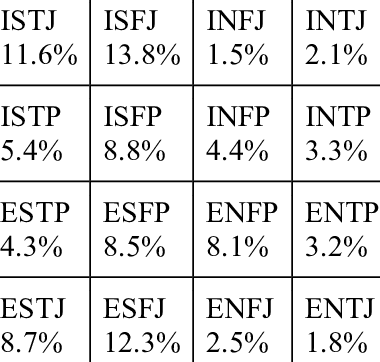
\includegraphics[width=\textwidth, height=10cm]{plots/association_rules.png}
    \caption[Myers-Briggs Type Indicator Breakdown]{Myers-Briggs Type Indicator Breakdown (Varona and Capretz, 2011)}
    \label{fig:ass_ch2}
\end{figure}

\pagebreak

\subsection{\textit{Contiguity}} 

Contiguity is an important aspect of the present interaction with housing insecurity. First, one of the main methods used to better understand rural areas is spatial autocorrelation. To conduct spatial autocorrelation, you must create a weights matrix and the type of contiguity you choose can have a significant impact on results. Second, proximity-based contiguity is an important aspect of capturing the inter-state nature of rural communities. Queen's contiguity is used to build the spatial weights matrix for analyzing the spatial autocorrelation of housing insecurity factors in rural areas. Queen's Contiguity looks for polygons that share a border. There are three general types of contiguity: Rook, Bishop, and Queen. Figure~\ref{fig:contiguity_relations} reflects the different boundaries considered by each type. As the figure shows, Queen contiguity allows for the highest number of shared borders.  This application is well-suited for Queen's contiguity because it best encapsulates the interconnected nature of rural areas.

 
\begin{figure}[htbp]
    \centering
    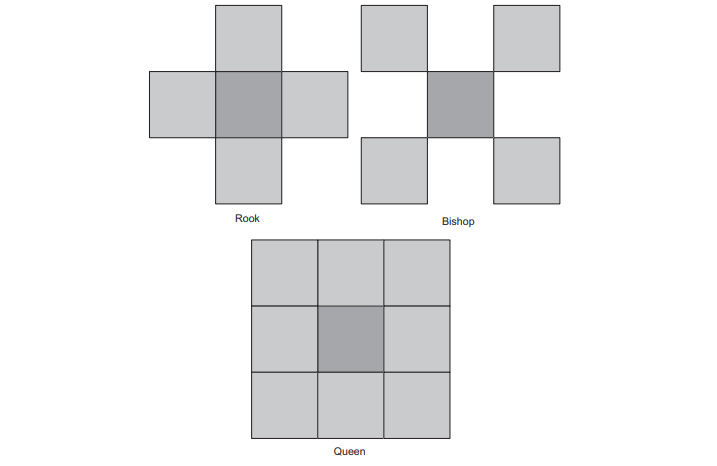
\includegraphics[width=\textwidth, height=8cm]{plots/contiguity.png}
    \caption[Types of Contiguity]{Types of Contiguity (Grubesic, 2008)}
    \label{fig:contiguity_relations}
\end{figure}

% gerrymandering article to explain how to deal with queen's contiguity in maps

% TODO: integrate this with Queen's Contiguity- give examples of how it matters IRL

These contiguity measures are used to analyze the connectivity of polygonal features, such as census tracts, in a geographic area \citep{grubesic_zip_2008}. Contiguity is an important part of creating the spatial weights matrix that underlies much of spatial analysis including Moran's \textit{I}. The spatial weights matrix is one of the most used measures of the influence that places have on each other \citep{bavaud_models_1998}. Shortly after the proposal of Moran's \textit{I} in 1950, the need to weight observations based on their influence was considered by the cartographer Arthur Robinson in 1956 \citep{getis_history_2008}. Since the 1960s, many researchers have attempted to properly represent spatial dependence with a spatial weights matrix, and the impact of one's definition of a neighbor on spatial results was recognized as well (\citealp{zhang_spatial_2012}; \citealp{getis_constructing_2004}). Since then, a variety of ways to generate a spatial weights matrix have been created including spatially contiguous neighbors, the length of shared borders divided by the perimeter, ranked distances, and \textit{n} nearest neighbors among others \citep{getis_constructing_2004}. Spatial weights and the definition of neighbors are closely related to Tobler's First Law of Geography, which is detailed in the following subsection. It should be noted that the chessboard concept of contiguity in Figure~\ref{fig:contiguity_relations} does not fully translate to the geographical space because of the inconsistencies in boundaries at different geographic levels.


In housing insecurity analyses that span state lines, overlooking neighboring communities can be unfair due to shared dependencies. To mitigate this, the analysis adopts proximity-based contiguity to encapsulate the interconnectedness of rural areas. Unlike the previously mentioned forms of contiguity, proximity-based contiguity defines adjacency based on proximity rather than a physical connection.  

\subsection{\textit{Spatial Autocorrelation}} 

Spatial autocorrelation is a method that enables researchers to account for the spatial patterns inherent in spatial data. Spatial autocorrelation is similar to correlation but rather than showing relationships between variables, it shows the correlation across georeferenced space \citep{getis_history_2008}. Generally, the concept refers to similar or dissimilar values producing a detectable pattern when placed on a map, often referred to as spatial clustering \citep{griffith_what_1992}. In an analysis of crops, \citet[74]{fisher_design_1935} noted that "patches in close proximity are commonly more alike... than those which are further apart". The idea known as spatial autocorrelation was not formalized until the proposal of Moran's \textit{I} in 1950, when it was referred to as spatial correlation (\citealp{moran_notes_1950}; \citealp{getis_history_2008}). Spatial autocorrelation is highly connected to Tobler's First Law of Geography. According to Tobler, "everything is related to everything else but near things are more related than distant things" \citep[236]{tobler_computer_1970}. Shortly after the proposal of Tobler's First Law of Geography, Cliff and Ord published a work titled Spatial Autocorrelation in 1973 which explicated and generalized Moran's earlier work \citep{getis_history_2008}. Since then, a variety of global and local spatial autocorrelation techniques have been proposed. For a more detailed history of spatial autocorrelation see \citet{fischer_spatial_2010}. Similar to other statistical tests, spatial autocorrelation is determined by rejecting the null hypothesis. \citet{de_jong_extreme_1984} highlight two general null hypotheses underlying spatial autocorrelation: 

\begin{itemize} 

\item The observations are mutually independent with a known or unknown distribution  

\item Each permutation of the observations $x_i$ is equally probable  

\end{itemize} 

 
When there is adequate information to reject the null hypothesis, an observation is said to be spatially autocorrelated. Figure \ref{fig:moran_ch2} provides a visual representation of spatial autocorrelation.\textcolor{white}{\citep{asgary_what_2020}}

\begin{figure}[htbp]
    \centering
    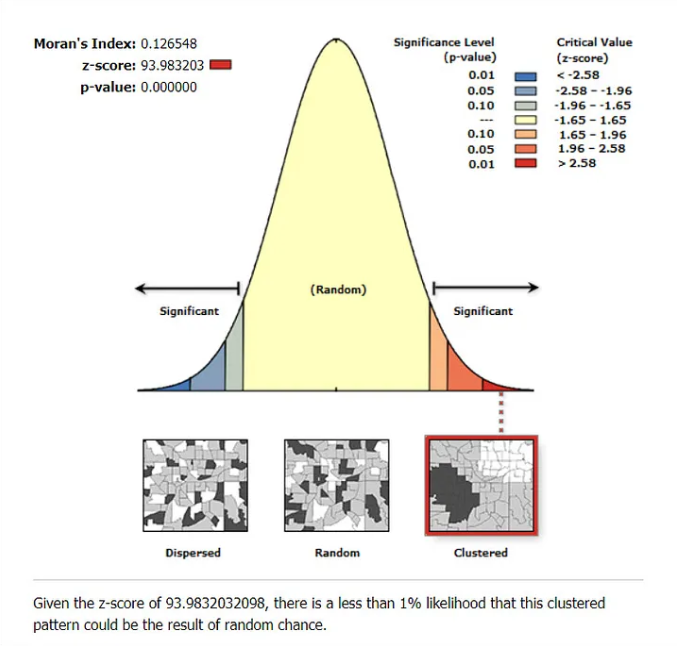
\includegraphics[width=\textwidth, height=10cm]{plots/moran_ch2.png}
    \caption[Spatial Autocorrelation Example]{Spatial Autocorrelation Example (Asgary, 2020)}
    \label{fig:moran_ch2}
\end{figure}

\pagebreak

Both local and global Moran's \textit{I} are used in this examination of housing insecurity. The primary difference between the two is that global Moran's \textit{I} measures spatial autocorrelation across an entire dataset while local Moran's \textit{I} assesses spatial autocorrelation at a local level. Three factors affect both global and local Moran's \textit{I} statistics according to \citet[320]{boots_global_2000} "the relative locations of \textit{i} and \textit{j}, the global average or local relative number of neighbours for \textit{i}, and the observed values of $x_i$, {$i \in \{1, \ldots, n\}$}". Several studies have applied spatial autocorrelation to housing insecurity. \citet{voss_county_2006} used Moran's \textit{I} to determine if there is spatial autocorrelation in county-level child poverty rates. \citet{curtis_spatial_2019} use spatial autocorrelation to analyze the clustering of industrial makeup (economic diversity) and poverty. \citet{brooks_advantages_2019} used Moran’s \textit{I} and Local indicators of Spatial Association statistics to further spatial inequality research. \citet{gleason_using_2021} use Local Indicators of Spatial Autocorrelation to analyze community vulnerability in rural areas in the state of Maine. These examples demonstrate a precedent for the use of spatial autocorrelation in the study of housing insecurity. 

 
\subsection{\textit{Multinomial Logistic Regression}} 

The final methodology used is multinomial logistic regression (MLR). The MLR is very similar to binomial logistic regression except the dependent variable contains more than two categories \citep{bayaga_multinomial_2010}. There are multiple usages of MLR. First is to determine the amount of variance in the dependent variable explained by the independent variables, second is to rank the importance of independent variables, third is to assess the interaction effects between variables, and finally is to understand the impact of control variables \citep{el-habil_application_2012}. The use of regression dates back to the 19th century with the proposal of least-squared regression although the challenge of finding the parameters in the equation of a straight line that optimally matches three or more points in the (x, y) plane has been recognized since at least the time of Galileo \citep{harter_method_1974}. Three different scholars published the method between 1805 and 1809 with Adrien Marie Legendre publishing it first in 1805, followed by Robert Adrian in 1808 or 1809, and Carl Friedrich Gauss in 1809 although Gauss claims to have used the method since 1795 \citep{stigler_gauss_1981}. Legendre's application was to determine the orbit of a comet given three observations on its longitude and latitude \citep[1]{legendre_nouvelles_1805}. Gauss similarly used the method for astronomical purposes \citep{davis_theory_2007}. Adrian's version of regression is more probabilistic than that of Legendre or Gauss \citep{dutka_robert_1990}. The logistic function underlying logistic regression was developed decades later by Pierre François Verhulst who developed it in a series of papers published between 1838 and 1847 \citep{cramer_origins_2003}. Decades later, Pearl and Reed published the logistic curve, unaware of Verhulst's work \citep{kingsland_refractory_1982}. See \citet{cramer_origins_2003} for a more detailed history of logistic regression. The MLR model used in this thesis was proposed by Berkson in 1944 and further developed by Cox in 1958 \citep{msaouel_medicine_2022}. MLR is similar to linear regression except it uses a maximum likelihood method where the fitted regression coefficients are used to maximize the probability of the observed result \citep{jackson_data_2002}. It does so by first transforming the dependent variable into a logit variable which is the natural log odds of the expected outcome either occurring or not occurring \citep{white_logistic_2013}. An example of the usage of multinomial logistic regression to housing insecurity could not be found, but regression is a popular technique among scholars. \citet{peters_typology_2009} used logistic regression in building their typology of American poverty. \citet{crandall_local_2004} used an ordinary least squares regression to measure the spatial concentration of poverty and poverty dynamics. \citet{wilson_rural_2016} use an ordinary least squares regression for modeling rural prosperity and federal expenditures. These similar applications demonstrate the usability of regression in the study of factors related to housing insecurity. 


\section{\textit{Summary}} 

Throughout this chapter, the 4 Cs of housing insecurity have been covered. It is important to highlight the interconnected nature of the 4 Cs. There is a significant overlap between each pillar of housing insecurity. Housing costs, housing type, and housing conditions are directly linked to the economic conditions of a household. These economic conditions are linked to the household factors that encapsulate their economic status. One's relation to the poverty level and education plays a significant role in housing accessibility and these factors are intrinsically linked to the context that they live in. Rural areas face numerous issues, some that align with problems in urban areas and some that do not such as the presence of mobile homes, economies built around single amenities, and large pockets of persistent poverty and prosperity. Any discussion on housing insecurity must consider the historical forces affecting modern-day race and poverty dynamics, and these forces relate to all aspects of life. When taken as a web, this model encompasses the wide-ranging socio-economic factors that surround housing insecurity. This chapter has also detailed the history, development, and fundamentals of the methods used in this thesis.  

 

\endinput 

 